
\section{Reuso de recursos no-ontológicos}
Los recursos no-ontológicos (NOR)\cite{ReusoRecursoNoOntologico} representan recursos de conocimiento cuya semántica no fue formalizada por una ontología. Estos NORs contienen conocimientos de un dominio en particular y representan algún grado de consenso colectivo. Estos recursos están presentes en forma de esquemas de clasificación, tesauros, diccionarios, etc. El principal desafío de los NORs es que la semántica no siempre está formalizada, osea legible por máquina, por lo tanto no son considerados ontologías formales según la definición adoptada.

En esta sección se desarrolla la búsqueda, evaluación y selección de recursos no-ontológicos que servirán como insumo para el desarrollo de la ontología.

\subsection{Búsqueda de recursos no-ontológicos }

En el proceso de búsqueda de documentación y estándares del dominio de Contrataciones Públicas se encontró que la DNCP implementa una API utilizando el estándar de publicación de datos de contrataciones públicas internacional \textit{Open Contracting Data Standard} (OCDS). La intención de la OCP fue crear un estándar que formaliza la sintaxis y no la semántica de cada concepto, a través de JSON Schema\cite{JSONSche10:online}, que es un vocabulario que permite anotar y validar documentos JSON. El estándar posee conceptos explícitamente definidos en lenguaje natural, por lo que la semántica esta definida pero no formalizada como ontología, por ello se lo consideró un recurso no-ontológico. Cabe recordar que cuando se habla de formal, se habla de legible por máquina. 

OCDS es un estándar amigable y flexible para estructurar información de Contrataciones Públicas y es mantenido por la OCP. El estándar describe qué, cuándo y cómo disponibilizar datos y documentos asociados en las diferentes fases del proceso de contratación. El proyecto promueve la divulgación y participación en las contrataciones públicas creando un estándar abierto de datos simple. OCDS posee un esquema de datos detallado de todos los conceptos así como también la estructura de los datos divulgados, dicho esquema esta disponible el sitio web del estándar \cite{OCDSReleaseSchema:online}. Este esquema ayuda a las personas a comprender todos los campos publicados. Además el estándar posee un guía de implementación de modo a facilitar la implementación\footnote{http://standard.open-contracting.org/latest/en/implementation/}.

En Paraguay,  el portal de datos abiertos de la DNCP \cite{DatosAbiDNCP:online}, organismo del estado que publica datos de los procesos de contrataciones , ha implementado el estándar y publica sus datos orientados a diferentes tipos de usuarios:


\begin{enumerate}
    \item Lista de datos. Con el fin de que los usuarios que necesitan ver, analizar y descargar en formato CSV los datos detallados de todos los registros de contrataciones.
    \item Visualizaciones de datos para usuarios que deseen ver estadísticas e información agregada.
    \item Una API para desarrolladores que permite manipular datos en formato JSON y JSON-LD de manera programática para cualquier otro uso.
    \item Plataforma de Contrataciones Electrónica, destinada a empresas y personas que deseen presentarse o conocer algún proceso de contratación.
\end{enumerate}

Los datos publicados poseen un diccionario de datos y una ontología creada por la DNCP, la cual sirve como contexto para la API desarrollada.Esto significa que la DNCP ya realizo un primer trabajo publicando sus datos en formato JSON-LD. Además la DNCP implementó una API siguiendo el estándar OCDS, que posee un esquema de publicación bien definido en JSON Schema.


\subsection{Evaluación de recursos no-ontológicos}
Se eligió el OCDS como recurso no-ontológico a evaluar puesto que el principal objetivo de este trabajo es que la ontología desarrollada sea compatible con dicho estándar de modelo de datos. Para realizar la evaluación se procedió a la extracción de las entradas léxicas, luego al cálculo de precisión y alcance para por último evaluar la factibilidad de reuso del recurso.  A continuación se explica en detalle cada paso.

\subsubsection{Extracción de entradas léxicas}
La meta de esta tarea es extraer las entradas léxicas de los recursos no-ontológicos. Para realizarla, es necesario tomar como entrada los recursos no-ontológicos y extraer sus entradas léxicas usando herramientas de extracción de terminología.	
			
Del esquema JSON de la versión 1 del OCDS se hizo una lista de todas las propiedades del mismo. Para este trabajo consideramos que cada propiedad del esquema consiste en una entrada léxica, donde una entrada léxica corresponde a un concepto o relación dentro del dominio de conocimiento. Asi como nuestra nuestro trabajo \footnote{http://bit.ly/ValdezBaezThesis}, se encontraron 142 propiedades, omitiendo las propiedades repetidas y datos transaccionales del estándar que no representan entradas léxicas, la lista se reduce a 114.

\subsubsection{Cálculo de precisión y alcance}

El objetivo de esta tarea es calcular la precisión de los recursos no-ontológicos candidatos. La precisión es una medida ampliamente utilizada en la recuperación de información y se define como la proporción del material recuperado que realmente es relevante. Esta tarea es llevada a cabo por los desarrolladores de software y los que utilicen la ontología teniendo como entrada las entradas léxicas extraídas de los recursos no-ontológicos y de la terminología reunida del ORSD. Para esto definimos los siguientes términos.

\begin{itemize}
    \item \textit{NOR Lexical Entries}  como el conjunto de entradas léxicas extraídas del recurso no ontológico.	
    \item \textit{ORSD Terminology} como el conjunto de términos identificados incluidos en el ORSD. 
\end{itemize}

Para obtener el número de términos de la especificación de requisitos de ontología (ORSDTerminology) se creó una lista unificada de todas las propiedades encontradas en el diccionario de datos del portal de datos abiertos de la DNCP.  Se encontraron 129 propiedades, de la misma manera que en el OCDS se omitieron propiedades repetidas y datos transaccionales, dejándonos con un total de 109 entradas léxicas. Éstas representan el dominio de conocimiento que se quiere representar con la ontología a construir.

\begin{table}[!htb]
\centering
\caption{Resumen de propiedades y entradas léxicas}
\label{resumen propiedades}
\begin{tabular}{|l|r|r|}
\hline
 & \textbf{Propiedades} & \textbf{Entradas léxicas}\\ \hline
 \textbf{OCDS} & 142 & 114\\ \hline
 \textbf{DNCP} & 129 & 109 \\ \hline
\end{tabular}
\end{table}

Para calcular la cobertura y la precisión del recurso no-ontológico se realizó la unión de términos equivalentes semánticamente. Dicha unión consiste en verificar términos equivalentes entre las entradas léxicas que estaban presentes en los requerimientos y en el recurso no-ontológico analizado. Cabe destacar que la metodología utilizada sólo tomó en cuenta las propiedades del esquema JSON del OCDS y el diccionario de datos de la API desarrollada por la DNCP, esto limita la cobertura, que podría ser más amplia si consideramos todos los términos del dominio de conocimiento. El resultado arrojó que existen 65 entradas léxicas comunes. Con estos datos se puede calcular la cobertura y la precisión a través de las  fórmulas \ref{eq:1} y \ref{eq:2}.

\begin{equation}
    \label{eq:1}
    Precision =  \frac{{NORLexicalEntries}\cap{ORDSTerminology} }{{NORLexicalEntries}}
\end{equation}

\begin{equation}
    \label{eq:3}
    Precision =  \frac{65}{114} = 0.5701754386
\end{equation}

\begin{equation}
    \label{eq:2}
     Coverage = \frac{{NORLexicalEntries}\cap{ORDSTerminology}}{{ORDSTerminology}}
\end{equation}

\begin{equation}
    \label{eq:4}
    Coverage =  \frac{65}{109} = 0.5963302752
\end{equation}

Esto da una cobertura de 0.59 y una precisión de 0.57.


\subsection{Selección del recurso no-ontológico}

Como se puede ver en el esquema del OCDS\footnote{http://standard.open-contracting.org/latest/en/schema/release/}, el mismo posee una especificación formal de la sintaxis de cada una de las propiedades, ya que por medio de un validador construido por la OCP\footnote{http://standard.open-contracting.org/validator/} podemos verificar si el objeto validado cumple con los requerimientos sintácticos de publicación del estándar.

También podemos observar que el estándar contiene explícitamente las descripciones de cada una de las propiedades del esquema JSON, por lo que posee información valiosa y consensuada de cada uno de los conceptos del dominio. Sin embargo, dicha información solamente es entendible por personas, no así procesable por máquinas, por lo que representa un recurso no-ontológico vital para el desarrollo de nuestra ontología.

Como se puede ver en el esquema del OCDS, el mismo posee una especificación formal de la sintaxis de cada una de las propiedades, ya que por medio de un validador construido por la OCP podemos verificar si el objeto validado cumple con los requerimientos sintácticos de publicación del estándar.

Las principales diferencias de cobertura entre los conceptos de la DNCP y la OCDS son que el segundo posee mayor información como es el caso de Periodo, Organización y Detalle de Contacto. También contempla los conceptos de Documentos, Transacciones, Hitos, una fase adicional de Implementación del Contrato y guarda el historial de cambios de todas las propiedades a través de las Adendas. Así también, el dominio de la DNCP agrega conceptos como Modificaciones de Contrato e información más detallada de Proveedores y Convocatorias. En la Figura \ref{img:coberturaontologia} se aprecia la intersección de los principales conceptos entre ambos dominios de conocimientos.

\begin{figure}[ht!]
    \centering
    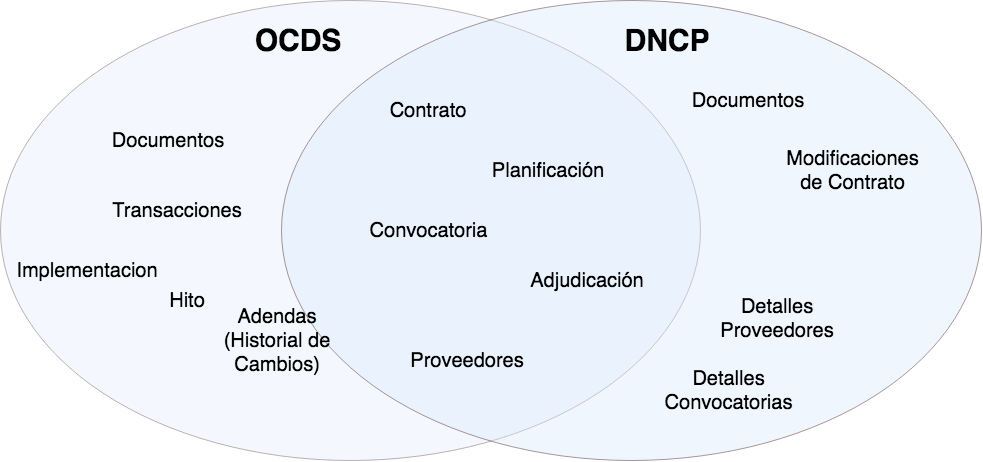
\includegraphics[width=150mm]{figuras/Diagramas-VennCobertura.png}
    \caption{Cobertura de los terminos de la DNCP y la OCDS}
    \label{img:coberturaontologia}
\end{figure}

    

El OCDS es implementado a nivel internacional, tiene una comunidad de colaboradores expertos en el dominio de distintos países, implementadores que dan al estándar una validez en cuanto a la aceptación de los términos, posee listas de correos y un sistema de gestión de cambios y mejoras activo en la plataforma Github\footnote{https://github.com/open-contracting/standard}. La intención de este trabajo es que la ontología sea utilizada no solamente por la DNCP sino por cualquier ente que realice procesos licitatorios, además, la DNCP está utilizando este estándar para publicación de datos orientados a desarrolladores. Con todo esto se aprecia que la cobertura es suficiente para utilizar el OCDS como recurso no-ontológico para nuestra ontología sacrificando así algunos detalles específicos de implementación local. Estos detalles más específicos se podrían cubrir a través del reuso y extensión de la ontología desarrollada en un futuro trabajo.
